\section{Lessons Learned}
\label{sec:lessons}

\FIXME{What are the lessons we have learned?}

\subsection{Pacing of Material}

\FIXME{Assignments with a duration of only one week.}

As recently as the spring semester of 2017, the pacing of material
was uneven and somewhat too fast.  The following are quotes from
end-of-semester student evaluations.
\begin{itemize}
\item ``The pace was inconsistent.''
\item ``It moved a little too fast in parts and wasn't always as
in-depth as I would've liked.''
\item ``We moved pretty quickly through material and I never felt like I had
time to fully grasp concepts because the assignments took so much time.''
\item ``The class moved too quickly.''
\item ``Assignments were too long for such short period of time.''
\end{itemize}
In reaction to these comments, we've evolved the course into the organization
that is described in Section~\ref{sec:weeks}.
For example, the networking module was (at least temporarily) retired
and the assembly language material was given more time (converted from a
2 week series into a 3 week series, without expanding the content).

In the most recent semester's student evaluations (spring 2018),
the results of the pace ratings are shown in Figure~\ref{fig:pace}
(using a 7-item Likert scale).
The mean score of 5.47 (std. dev. of 1.41)
is very close to the department's average of
5.66, and a substantial improvement from the mean score of 4.51
for the course in spring of 2017.

\begin{figure}[ht]
\centering
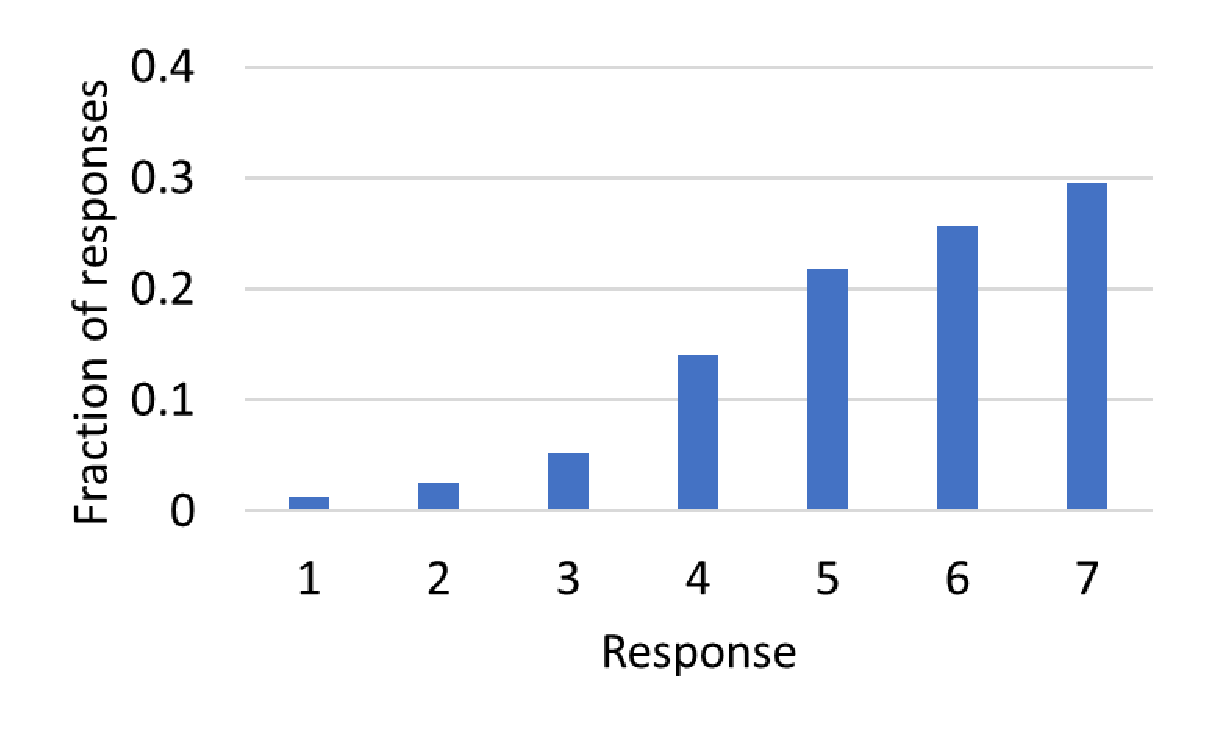
\includegraphics[width=\columnwidth]{pace}
\caption{Student ratings of statement, ``The material was covered
at a reasonable pace''  (scoring: 1 - Strongly Disagree, 7 - Strongly Agree).}
\label{fig:pace}
\end{figure}

\subsection{Analysis Problems}

Based on commentary in the literature that posits the benefits of
analysis problems in the context of design courses~\cite{wjbo01},
we were concerned that the present
course doesn't have sufficient analysis content (i.e., the bulk of
studio questions and assignment questions are design questions rather
than analysis questions).

To test this theory, we generated an additional set of analysis problems,
designed to be helpful in preparing students for the third exam, and
made them available to students one week prior to the exam.  To provide
an incentive for the students to attempt them, students were told that
there would be a small amount of extra credit for those that did well.

We then compared scores for the two groups of students, those who did
attempt the extra credit exercise and those who did not.  The results
of this comparison are shown in Figure~\ref{fig:scores}.
There clearly is a correlation between overall course grade and
whether or not a student attempted the extra exercise.
Those who attemped the extra exercise scored over 4\% higher overall
(the scores presented exclude the extra credit provided from the
exercise).  This is statistically significant at $p = 0.02$ (non-paired data).

\begin{figure}[ht]
\centering
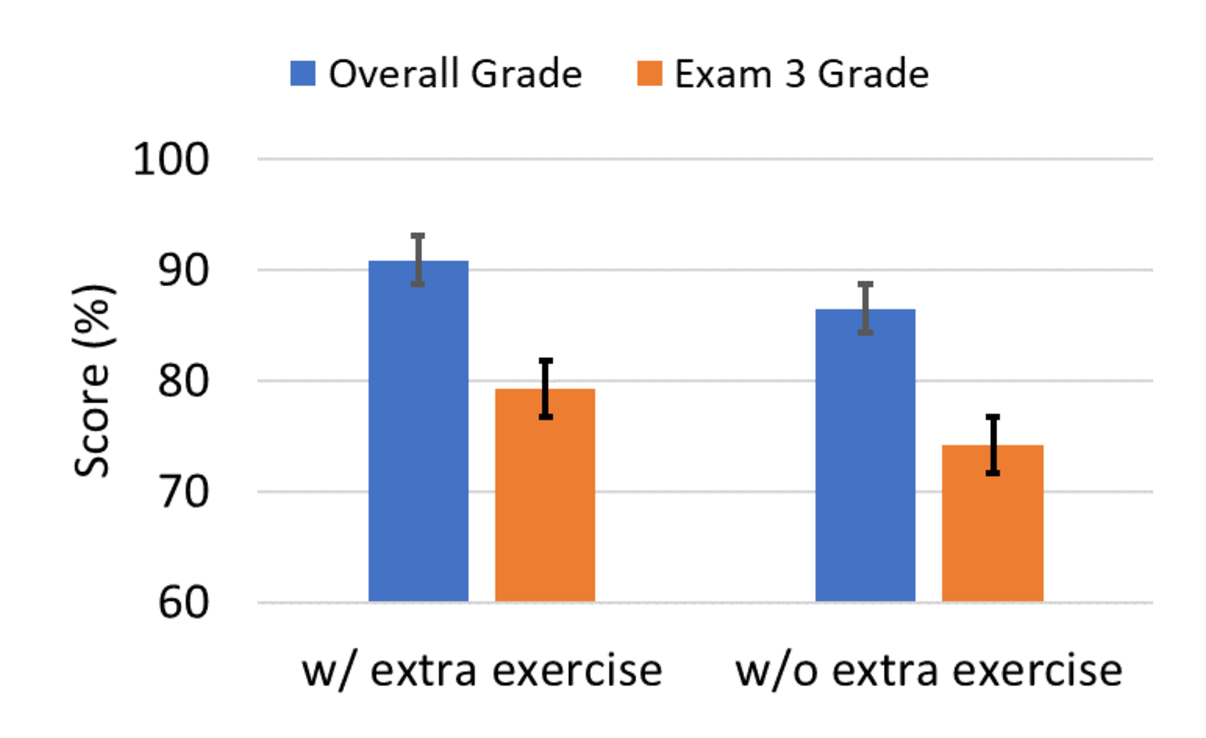
\includegraphics[width=\columnwidth]{scores}
\caption{Relationship between overall scores and exam~3 scores
with and without the extra exercise. The bars indicate mean score and
the whiskers indicate standard error.}
\label{fig:scores}
\end{figure}

When we examine the scores on exam~3, however, the story is different.
While the mean score differential is similar (at 5\% in this case), the
variability in scores is wide enough that this result is not
statistically significant ($p = 0.11$, non-paired data), so we cannot
rule out the null hypothesis that the difference in the means is
due to chance.

Our current opinion is that the correlation seen in the overall scores
is nothing as specific as a single exercise, but is more likely due to the
fact that better students (more likely to achieve a higher score prior
to the availability of an optional exercise) are also more likely than
their peers to take advantage of an optional exercise, especially when
it provides extra credit.

Going forward, we are still interested in whether or not additional
analysis problems can help students learn the material better, and will
likely pursue it by altering the mix of analysis vs.~design problems
within the studio exercises.

\subsection{Logistics}

\FIXME{Reintroduction of "lecture" (actually recitation).}

In general, the logistics of the course haven't been as smooth as they could be.
A couple quotes from recent student evaluations (spring 2018):
\begin{itemize}
\item ``More structure and organization, use more difficult examples when
teaching the material since the assignments were a lot harder than
the given examples.''
\item ``It needs more organization.''
\end{itemize}
This past semester we didn't do as good a job as we should have
in communicating due dates, etc. A number of the specifics on the calendar
were filled out (made available to the students) as the semester proceeded.
In retrospect, this was a mistake, as a number of things didn't make it on
to the calendar early enough for everyone to see them.

The removal of a live lecture session in favor of on-line videos has also been
a challenge for some students. Since videos are static content, there is an
extra layer of effort that students must take if they do not understand the
presented concepts or need additional explanation. Interactions with professors
are also fewer and farther between as students are spread out across multiple
computer labs instead of meeting as a single, large group.

In the fall of 2017, we introduced a recitation section to address these issues.
The recitation sections would occur after the weekly studio, but before the weekly
assignment was due, so students could ask questions about topics they had
seen in the on-line videos and studio. The effect of these recitaiton sessions
was somewhat mixed, as shown by comments on student evaluations:
\begin{itemize}
\item ``I only attended a handful of the recitation, specifically when I was
confused on a topic, and every time I came my questions were answered and
it was very helpful."
\item ``Kind of a waste of time."
\end{itemize}

A common complaint about recitation sessions is that they were short and
unstructured. While the recitation sessions were intended to be loosely
structured and student-driven by design, a more structured approach with
pre-prepared review questions and practice problems may prove to be
more beneficial for students.

Like many computer science programs, we are seeing an increase in
the number of students enrolled in our courses. This led to a bottleneck
during assignment submission time, as having students demo their work
took time and there would also inevitably be a number of students who had
last minute problems that needed to be solved before they could submit their
assignment. This combination was putting a strain on our TAs, and students
were having difficulty getting the help that they needed on these busy days.

This past semester, the professors of the course started holding office hours in
one of the nearby computer labs during these busy times. Students who had
problems with that week's assignment had a direct line to someone who could
help them, which freed up the TAs to focus on demoing completed assignments.
This setup greatly increased the efficiency of assignment submissions and will
likely be continued in future semesters.
